\documentclass[11pt,a4paper]{report}
\usepackage[textwidth=37em,vmargin=30mm]{geometry}
\usepackage{calc,xunicode,amsmath,amssymb,paralist,enumitem,tabu,booktabs,datetime2,xeCJK,xeCJKfntef,listings}
\usepackage{tocloft,fancyhdr,tcolorbox,xcolor,graphicx,eso-pic,xltxtra,xelatexemoji}

\newcommand{\envyear}[0]{2024}
\newcommand{\envdatestr}[0]{2024-11-17}
\newcommand{\envfinaldir}[0]{webdb/2024/20241117/final}

\usepackage[hidelinks]{hyperref}
\hypersetup{
    colorlinks=false,
    pdfpagemode=FullScreen,
    pdftitle={Web Digest - \envdatestr}
}

\setlength{\cftbeforechapskip}{10pt}
\renewcommand{\cftchapfont}{\rmfamily\bfseries\large\raggedright}
\setlength{\cftbeforesecskip}{2pt}
\renewcommand{\cftsecfont}{\sffamily\small\raggedright}

\setdefaultleftmargin{2em}{2em}{1em}{1em}{1em}{1em}

\usepackage{xeCJK,xeCJKfntef}
\xeCJKsetup{PunctStyle=plain,RubberPunctSkip=false,CJKglue=\strut\hskip 0pt plus 0.1em minus 0.05em,CJKecglue=\strut\hskip 0.22em plus 0.2em}
\XeTeXlinebreaklocale "zh"
\XeTeXlinebreakskip = 0pt


\setmainfont{Brygada 1918}
\setromanfont{Brygada 1918}
\setsansfont{IBM Plex Sans}
\setmonofont{JetBrains Mono NL}
\setCJKmainfont{Noto Serif CJK SC}
\setCJKromanfont{Noto Serif CJK SC}
\setCJKsansfont{Noto Sans CJK SC}
\setCJKmonofont{Noto Sans CJK SC}

\setlength{\parindent}{0pt}
\setlength{\parskip}{8pt}
\linespread{1.15}

\lstset{
	basicstyle=\ttfamily\footnotesize,
	numbersep=5pt,
	backgroundcolor=\color{black!5},
	showspaces=false,
	showstringspaces=false,
	showtabs=false,
	tabsize=2,
	captionpos=b,
	breaklines=true,
	breakatwhitespace=true,
	breakautoindent=true,
	linewidth=\textwidth
}






\newcommand{\coverpic}[2]{
    % argv: itemurl, authorname
    Cover photo by #2~~(\href{#1}{#1})
}
\newcommand{\makeheader}[0]{
    \begin{titlepage}
        % \newgeometry{hmargin=15mm,tmargin=21mm,bmargin=12mm}
        \begin{center}
            
            \rmfamily\scshape
            \fontspec{BaskervilleF}
            \fontspec{Old Standard}
            \fontsize{59pt}{70pt}\selectfont
            WEB\hfill DIGEST
            
            \vfill
            % \vskip 30pt
            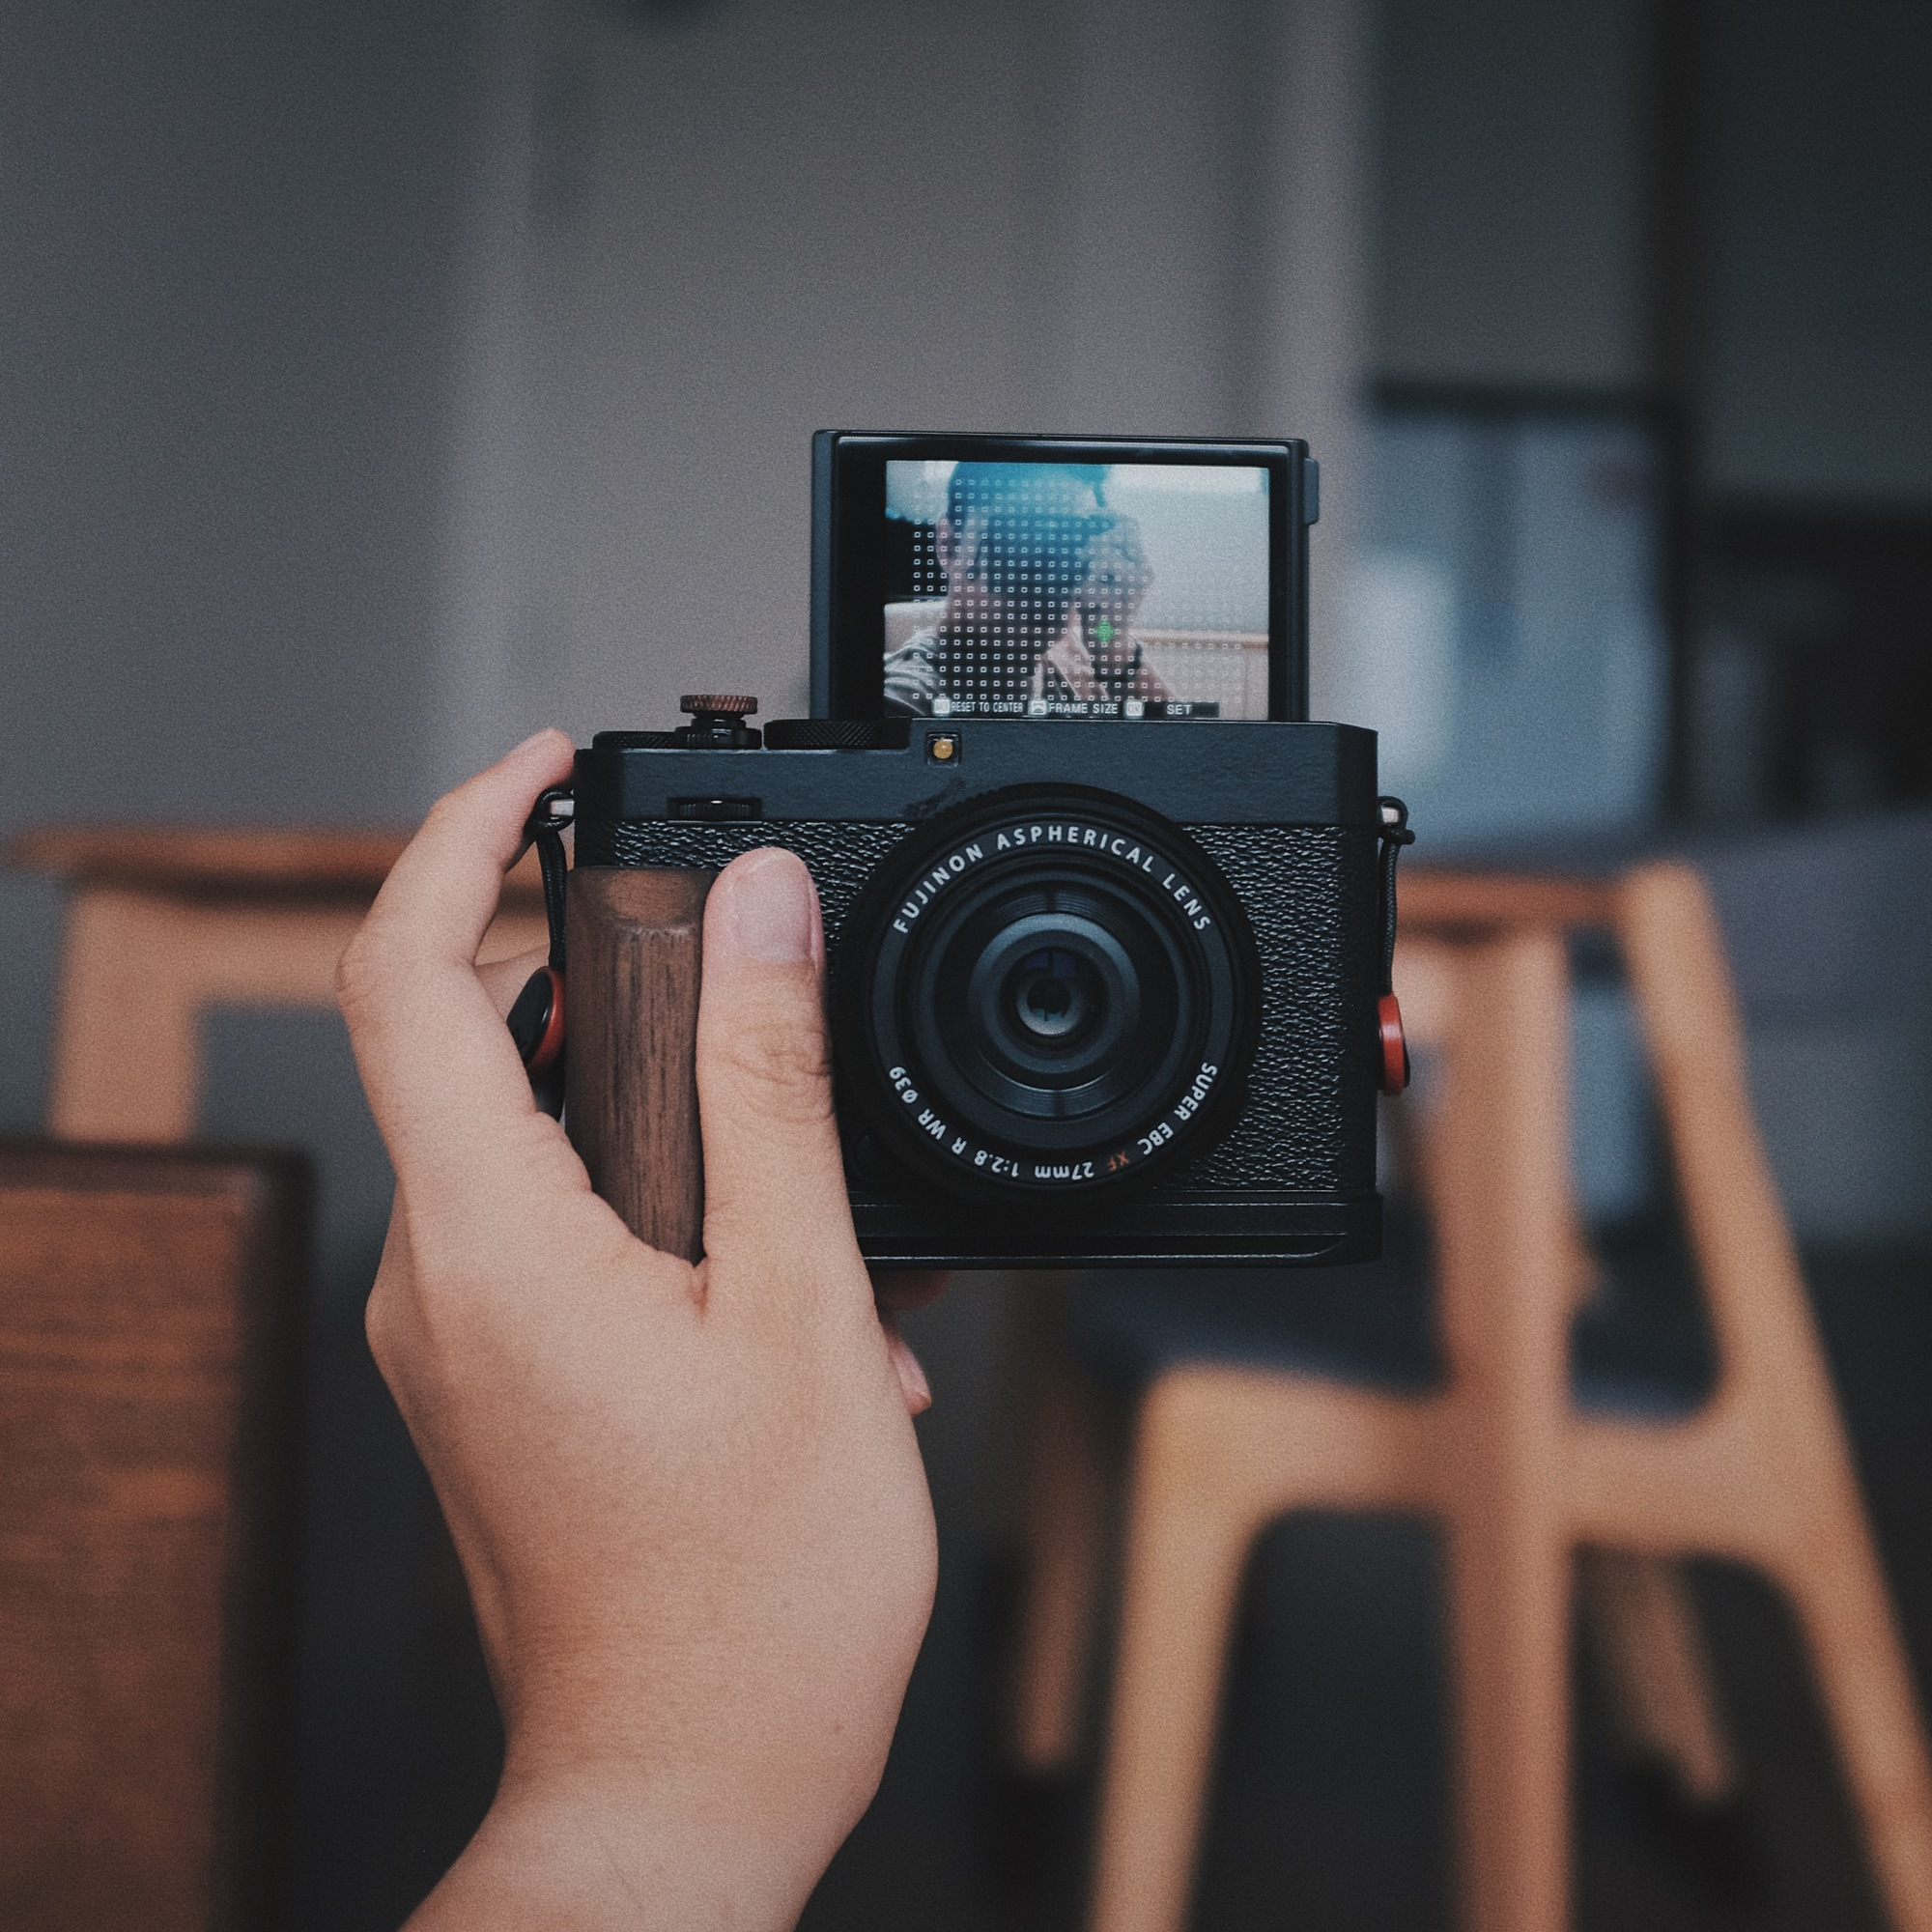
\includegraphics[width=\linewidth]{\envfinaldir/coverpic-prod.jpg}\par
            % \vskip 30pt
            \vfill

            \normalsize\rmfamily\scshape
            \copyright{} The Web Digest Project \hfill\large \envdatestr
        \end{center}
    \end{titlepage}
    % \restoregeometry
}
\newcommand{\simplehref}[1]{%
    \textcolor{blue!80!green}{\href{#1}{#1}}%
}
\renewcommand{\contentsname}{\center\Huge\sffamily\bfseries Contents\par\vskip 20pt}
\newcounter{ipartcounter}
\setcounter{ipartcounter}{0}
\newcommand{\ipart}[1]{
    % \vskip 20pt
    \clearpage
    \stepcounter{ipartcounter}
    \phantomsection
    \addcontentsline{toc}{chapter}{#1}
    % \begin{center}
    %     \Huge
    %     \sffamily\bfseries
    %     #1
    % \end{center}
    % \vskip 20pt plus 7pt
}
\newcounter{ichaptercounter}
\setcounter{ichaptercounter}{0}
\newcommand{\ichapter}[1]{
    % \vskip 20pt
    \clearpage
    \stepcounter{ichaptercounter}
    \phantomsection
    \addcontentsline{toc}{section}{\numberline{\arabic{ichaptercounter}}#1}
    \begin{center}
        \Huge
        \sffamily\bfseries
        #1
    \end{center}
    \vskip 20pt plus 7pt
}
\newcommand{\entrytitlefont}[1]{\subsection*{\raggedright\Large\sffamily\bfseries#1}}
\newcommand{\entryitemGeneric}[2]{
    % argv: title, url
    \parbox{\linewidth}{
        \entrytitlefont{#1}\par\vskip 5pt
        \footnotesize\ttfamily\mdseries
        \simplehref{#2}
    }\vskip 11pt plus 11pt minus 1pt
}
\newcommand{\entryitemGithub}[3]{
    % argv: title, url, desc
    \parbox{\linewidth}{
        \entrytitlefont{#1}\par\vskip 5pt
        \footnotesize\ttfamily\mdseries
        \simplehref{#2}\par\vskip 5pt
        \small\rmfamily\mdseries#3
    }\vskip 11pt plus 11pt minus 1pt
}
\newcommand{\entryitemAp}[3]{
    % argv: title, url, desc
    \parbox{\linewidth}{
        \entrytitlefont{#1}\par\vskip 5pt
        \footnotesize\ttfamily\mdseries
        \simplehref{#2}\par\vskip 5pt
        \small\rmfamily\mdseries#3
    }\vskip 11pt plus 11pt minus 1pt
}
\newcommand{\entryitemHackernews}[3]{
    % argv: title, hnurl, rawurl
    % \parbox{\linewidth}{
    %     \entrytitlefont{#1}\par\vskip 5pt
    %     \footnotesize\ttfamily\mdseries
    %     \simplehref{#3}\par
    %     \textcolor{black!50}{\href{#2}{#2}}
    % }\vskip 11pt plus 11pt minus 1pt
    \begin{minipage}{\linewidth}
            \entrytitlefont{#1}\par\vskip 5pt
            \footnotesize\ttfamily\mdseries
            \simplehref{#3}\par
            \textcolor{black!50}{\href{#2}{#2}}
    \end{minipage}\par\vskip 11pt plus 11pt minus 1pt
}







\begin{document}

\makeheader

\tableofcontents\clearpage




\ipart{Developers}
\ichapter{Hacker News}
\entryitemTwoLinks{Bluesky is currently gaining more than 1M users a day}{https://news.ycombinator.com/item?id=42159713}{https://bsky.jazco.dev/stats}

\entryitemTwoLinks{Four dead in fire as Tesla doors fail to open after crash}{https://news.ycombinator.com/item?id=42158391}{https://myelectricsparks.com/four-dead-tesla-doors-fail-open-crash-fire/}

\entryitemTwoLinks{James Webb Space Telescope finds evidence for alternate theory of gravity}{https://news.ycombinator.com/item?id=42158130}{https://thedebrief.org/james-webb-space-telescope-finds-stunning-evidence-for-alternate-theory-of-gravity/}

\entryitemTwoLinks{SICP: The only computer science book worth reading twice? (2010)}{https://news.ycombinator.com/item?id=42157558}{https://simondobson.org/2010/05/14/cs-book-worth-reading-twice/}

\entryitemTwoLinks{Ask HN: What open source projects need help?}{https://news.ycombinator.com/item?id=42157556}{https://news.ycombinator.com/item?id=42157556}

\entryitemTwoLinks{Two galaxies aligned in a way where their gravity acts as a compound lens}{https://news.ycombinator.com/item?id=42157335}{https://phys.org/news/2024-11-astronomers-galaxies-aligned-gravity-compound.html}

\entryitemTwoLinks{M4 Macs can't virtualise older macOS}{https://news.ycombinator.com/item?id=42157086}{https://eclecticlight.co/2024/11/14/m4-macs-cant-virtualise-older-macos/}

\entryitemTwoLinks{Show HN: I built a(nother) house optimized for LAN parties}{https://news.ycombinator.com/item?id=42156977}{https://lanparty.house/}

\entryitemTwoLinks{Casio has released a ring in the form of its iconic watch}{https://news.ycombinator.com/item?id=42156680}{https://www.theverge.com/2024/11/15/24297261/casio-smart-ring-digital-watch-crw-001-1jr}

\entryitemTwoLinks{Treating bullying as everyone's problem reduces incidence in primary schools}{https://news.ycombinator.com/item?id=42156640}{https://phys.org/news/2024-11-bullying-problem-incidence-primary-schools.html}

\entryitemTwoLinks{YC is wrong about LLMs for chip design}{https://news.ycombinator.com/item?id=42156516}{https://www.zach.be/p/yc-is-wrong-about-llms-for-chip-design}

\entryitemTwoLinks{Yggdrasil Network}{https://news.ycombinator.com/item?id=42155780}{https://yggdrasil-network.github.io/}

\entryitemTwoLinks{Kyanos: eBPF-based network issue analysis tool}{https://news.ycombinator.com/item?id=42154583}{https://github.com/hengyoush/kyanos}

\entryitemTwoLinks{Llama-OCR: Document to Markdown}{https://news.ycombinator.com/item?id=42154410}{https://llamaocr.com/}

\entryitemTwoLinks{Netflix buffering issues: Boxing fans complain about Jake Paul vs. Mike Tyson}{https://news.ycombinator.com/item?id=42153953}{https://www.sportingnews.com/us/boxing/news/netflix-buffering-livestream-issues-boxing-jake-paul-mike-tyson/327ee972d4b14d90cc370461}

\entryitemTwoLinks{Tsugaru OS – A New Free FM-Towns OS}{https://news.ycombinator.com/item?id=42153535}{https://github.com/captainys/FreeTOWNSOS}

\entryitemTwoLinks{M4 MacBook Pros use a quantum dot (QD) film rather than a red KSF phosphor film}{https://news.ycombinator.com/item?id=42152928}{https://twitter.com/DSCCRoss/status/1857208745014776215}

\entryitemTwoLinks{Consuming the Bluesky firehose for less than \$2.50/mo}{https://news.ycombinator.com/item?id=42152362}{https://bsky.bad-example.com/consuming-the-firehose-cheaply/}

\entryitemTwoLinks{Non-elementary group-by aggregations in Polars vs pandas}{https://news.ycombinator.com/item?id=42152076}{https://labs.quansight.org/blog/dataframe-group-by}

\entryitemTwoLinks{FTC to launch investigation into Microsoft's cloud business}{https://news.ycombinator.com/item?id=42152068}{https://arstechnica.com/tech-policy/2024/11/ftc-to-launch-investigation-into-microsofts-cloud-business/}\ichapter{Phoronix}
\entryitemGeneric{\hskip 0pt{}Google Engineer Proposes "Page Detective" As New Kernel Debugging Tool}{https://www.phoronix.com/news/Linux-Page-Detective-RFC}

\entryitemGeneric{\hskip 0pt{}TUXEDO Computers Relicenses Some Of Their Drivers To GPLv2}{https://www.phoronix.com/news/TUXEDO-Some-Drivers-GPLv2}

\entryitemGeneric{\hskip 0pt{}Rustls 0.23.17 Brings More Performance Improvements}{https://www.phoronix.com/news/Rustls-0.23.17-Released}

\entryitemGeneric{\hskip 0pt{}GCC 15 Moves C Default Language Version To C23}{https://www.phoronix.com/news/GCC-15-Default-C23}

\entryitemGeneric{\hskip 0pt{}Linux 6.13 Introducing New Rust File Abstractions}{https://www.phoronix.com/news/Linux-6.13-Rust-File-Abstract}

\entryitemGeneric{\hskip 0pt{}KDE Developers Spent The Week Fixing Bugs \& Polishing}{https://www.phoronix.com/news/KDE-Plasma-6.3-Nov-Progress}

\entryitemGeneric{\hskip 0pt{}systemd 257-rc2 Released With New systemd-keyutil Tool}{https://www.phoronix.com/news/systemd-257-rc2}

\entryitemGeneric{\hskip 0pt{}Valve Releases Half-Life 2 20th Anniversary Update}{https://www.phoronix.com/news/Half-Life-2-20th-Anniversary}

\entryitemGeneric{\hskip 0pt{}Tmpfs Adding Case Insensitive Support For Wine / Steam Play \& Flatpaks}{https://www.phoronix.com/news/Linux-6.13-Tmpfs-Case-Folding}


\ipart{Developers~~~~(zh-Hans)}
\ichapter{Solidot}
\entryitemGeneric{\hskip 0pt{}NSO Group 而不是政府客户运营着间谍软件}{https://www.solidot.org/story?sid=79793}

\entryitemGeneric{\hskip 0pt{}Valve 庆祝《半条命2》二十周年,游戏限时免费}{https://www.solidot.org/story?sid=79792}

\entryitemGeneric{\hskip 0pt{}Yandex 禁止中国 IP 搜索图片和视频}{https://www.solidot.org/story?sid=79791}

\entryitemGeneric{\hskip 0pt{}调查显示 AI 热在降温}{https://www.solidot.org/story?sid=79790}

\entryitemGeneric{\hskip 0pt{}OpenAI、Google 和 Anthropic 在构建更先进 AI 模型上遭遇瓶颈}{https://www.solidot.org/story?sid=79789}

\entryitemGeneric{\hskip 0pt{}网信办发布《移动互联网未成年人模式建设指南》}{https://www.solidot.org/story?sid=79788}

\entryitemGeneric{\hskip 0pt{}《半条命2》迎来二十周年,社区开发者制作 RTX 版本}{https://www.solidot.org/story?sid=79787}

\entryitemGeneric{\hskip 0pt{}美团单车和哈啰单车在郑州市暂停运营}{https://www.solidot.org/story?sid=79786}

\entryitemGeneric{\hskip 0pt{}研究发现错过截止日期会导致他人更苛刻的评价你的工作}{https://www.solidot.org/story?sid=79785}

\entryitemGeneric{\hskip 0pt{}美国黑客因窃取 Bitfinex 比特币被判五年}{https://www.solidot.org/story?sid=79784}

\entryitemGeneric{\hskip 0pt{}中国的机器人革命迫使劳动力作出改变}{https://www.solidot.org/story?sid=79783}

\entryitemGeneric{\hskip 0pt{}韩国研究人员重新发明轮子}{https://www.solidot.org/story?sid=79782}

\entryitemGeneric{\hskip 0pt{}OpenMP 6.0 释出}{https://www.solidot.org/story?sid=79781}

\entryitemGeneric{\hskip 0pt{}Meta 因违反欧盟反垄断规定被罚 8.4 亿美元}{https://www.solidot.org/story?sid=79780}

\entryitemGeneric{\hskip 0pt{}因使用盗版软件期刊撤下了两篇论文}{https://www.solidot.org/story?sid=79779}

\entryitemGeneric{\hskip 0pt{}洋葱新闻拍下了 InfoWars}{https://www.solidot.org/story?sid=79778}

\entryitemGeneric{\hskip 0pt{}意大利出人意料的成为间谍软件的主要供应国}{https://www.solidot.org/story?sid=79777}

\entryitemGeneric{\hskip 0pt{}AI 只能完成高等数学新测试问题的不到 2\%}{https://www.solidot.org/story?sid=79776}

\entryitemGeneric{\hskip 0pt{}GOG 宣布了经典游戏的保存计划}{https://www.solidot.org/story?sid=79775}

\entryitemGeneric{\hskip 0pt{}Steam 停止支持 Windows 7 和 Windows 8}{https://www.solidot.org/story?sid=79774}\ichapter{V2EX}
\entryitemGeneric{\hskip 0pt{}[MacBook Air] 关于合盖外接显示器的声音问题}{https://www.v2ex.com/t/1090207}

\entryitemGeneric{\hskip 0pt{}[问与答] 为什么很多``知识付费''博主讲的内容很浅废话占 9 成,但确实能赚钱?}{https://www.v2ex.com/t/1090206}

\entryitemGeneric{\hskip 0pt{}[Apple] macOS Finder 侧边栏中 SMB 共享的图标有办法改吗?}{https://www.v2ex.com/t/1090205}

\entryitemGeneric{\hskip 0pt{}[问与答] 有 123 网盘资源搜索的站点吗}{https://www.v2ex.com/t/1090204}

\entryitemGeneric{\hskip 0pt{}[程序员] iOS 求推荐一本你看过最为经典的书(Apple 开发相关的)}{https://www.v2ex.com/t/1090203}

\entryitemGeneric{\hskip 0pt{}[Apple] 有办法让 2 台苹果电脑不插拔雷电线切换一个雷电扩展坞么? type-c 切换器好像不行?}{https://www.v2ex.com/t/1090202}

\entryitemGeneric{\hskip 0pt{}[分享发现] ios 端的 parsec 由国人接手了一个开源版本}{https://www.v2ex.com/t/1090201}

\entryitemGeneric{\hskip 0pt{}[程序员] 创建个人题库系统}{https://www.v2ex.com/t/1090199}

\entryitemGeneric{\hskip 0pt{}[Linux] 哪个 Linux 发新版本支持 Darwin(Mac OS)的键位?}{https://www.v2ex.com/t/1090198}

\entryitemGeneric{\hskip 0pt{}[云计算] AWS 的入站流量为何是不收费的,只有出站才收费?}{https://www.v2ex.com/t/1090197}

\entryitemGeneric{\hskip 0pt{}[Apple] 买了 Macbook Pro M4 Pro!鸟枪换炮,再也没有拖延的借口了!}{https://www.v2ex.com/t/1090196}

\entryitemGeneric{\hskip 0pt{}[宽带症候群] 软路由和光猫兼容性}{https://www.v2ex.com/t/1090195}

\entryitemGeneric{\hskip 0pt{}[iPhone] 老安卓用户认为右滑返回是 iPhone 最辣鸡的功能}{https://www.v2ex.com/t/1090194}

\entryitemGeneric{\hskip 0pt{}[Android] 2024 年 11 月。性能足够强大的小屏安卓手机推荐}{https://www.v2ex.com/t/1090193}

\entryitemGeneric{\hskip 0pt{}[求职] 深圳求捞}{https://www.v2ex.com/t/1090192}

\entryitemGeneric{\hskip 0pt{}[分享创造] [网站自荐] Sound Box 专业的高颜值免费在线情境音效平台,提供多种自然环境音效以及白噪音,帮助用户打造完美的声音空间。无论是为了专注工作、放松心情,还是助眠解压,都能找到最适合的声音组合。}{https://www.v2ex.com/t/1090191}

\entryitemGeneric{\hskip 0pt{}[问与答] 有什么网盘不开会员的容量高而且可以分享文件?}{https://www.v2ex.com/t/1090190}

\entryitemGeneric{\hskip 0pt{}[分享创造] [分享] 一个基于 LLaMA 的 AI 聊天伴侣应用}{https://www.v2ex.com/t/1090189}

\entryitemGeneric{\hskip 0pt{}[Android] 剪切板里出现这段话"每一个梦想的实现都需要耐心与坚持......果实乩岸此墅抛磅"请问有碰到相同情况的吗?}{https://www.v2ex.com/t/1090188}

\entryitemGeneric{\hskip 0pt{}[Python] / 然后 math.floor 和 // 结果不一致……求教数据格式转换机制}{https://www.v2ex.com/t/1090186}

\entryitemGeneric{\hskip 0pt{}[Apple] AAPL ID 加入家庭的邀请邮件是由 AAPL 官方发送 还是 家长发送?}{https://www.v2ex.com/t/1090185}

\entryitemGeneric{\hskip 0pt{}[程序员] XXL-JOB v2.4.2 发布 | 分布式任务调度平台}{https://www.v2ex.com/t/1090184}

\entryitemGeneric{\hskip 0pt{}[游戏] 解决 Steam 下载速度为 0 或者很慢的方法}{https://www.v2ex.com/t/1090182}

\entryitemGeneric{\hskip 0pt{}[问与答] 每月打印 500 页左右,有啥打印机推荐?}{https://www.v2ex.com/t/1090181}

\entryitemGeneric{\hskip 0pt{}[问与答] 显示器只有一个 c 口,想插一个 mac mini 和一个 macbook 有没有什么办法}{https://www.v2ex.com/t/1090179}

\entryitemGeneric{\hskip 0pt{}[问与答] 双十一剁手了绿联 DXP4800,怎么将现有的群晖 220j 的数据转移到绿联上?}{https://www.v2ex.com/t/1090176}

\entryitemGeneric{\hskip 0pt{}[生活] 哎,运营商逐步关闭了一些基站,现在手机直接无服务了。}{https://www.v2ex.com/t/1090175}

\entryitemGeneric{\hskip 0pt{}[全球工单系统] 百度网盘 Mac 版本 4.39.6 (177)}{https://www.v2ex.com/t/1090174}

\entryitemGeneric{\hskip 0pt{}[Apple] 香港教育优惠要怎么寄到大陆?}{https://www.v2ex.com/t/1090173}

\entryitemGeneric{\hskip 0pt{}[程序员] 开发时怎么找到自己想要的 api}{https://www.v2ex.com/t/1090172}

\entryitemGeneric{\hskip 0pt{}[加密货币] 从 2 万到 10 万美金的成长之路}{https://www.v2ex.com/t/1090171}

\entryitemGeneric{\hskip 0pt{}[问与答] macOS bambu studio 查看打印机视频监控,提示播放器异常,请重新安装,有啥办法可以解决}{https://www.v2ex.com/t/1090169}

\entryitemGeneric{\hskip 0pt{}[Apple] m1 编译了 llvm,不由得感叹尚能饭否!}{https://www.v2ex.com/t/1090168}

\entryitemGeneric{\hskip 0pt{}[Netflix] 关于 Netflix 手机号验证}{https://www.v2ex.com/t/1090166}

\entryitemGeneric{\hskip 0pt{}[VPS] 国内 VPS 访问 git,docker 速度如何加速}{https://www.v2ex.com/t/1090165}

\entryitemGeneric{\hskip 0pt{}[问与答] 现在程序员用静电容键盘的多么}{https://www.v2ex.com/t/1090164}

\entryitemGeneric{\hskip 0pt{}[问与答] ipfs 和传统的 p2p bt(pt) 有什么本质上的不同吗?运营商也是可以清楚可见的吧? 是否更私密?}{https://www.v2ex.com/t/1090163}

\entryitemGeneric{\hskip 0pt{}[问与答] 如何使用 ESP32 开发板发射了 多个伪装成美国 WiFi 的信号?}{https://www.v2ex.com/t/1090162}

\entryitemGeneric{\hskip 0pt{}[Bitcoin] 现在交易所的 usdt 提到香港银行的线上最佳中转路径是什么?}{https://www.v2ex.com/t/1090161}

\entryitemGeneric{\hskip 0pt{}[程序员] XXL-API v1.2.0 发布 | API 管理平台}{https://www.v2ex.com/t/1090159}

\entryitemGeneric{\hskip 0pt{}[iPad] 上海哪里有靠谱的维修 iPad 的地方, v 友们推荐下}{https://www.v2ex.com/t/1090157}

\entryitemGeneric{\hskip 0pt{}[macOS] menu bar 上图标总是莫名其妙消失一部分, 有时候又会出现, 重启也有概率恢复, 怎么解?}{https://www.v2ex.com/t/1090155}

\entryitemGeneric{\hskip 0pt{}[分享创造] 刚刚上线了个人第 5 个网站-宝宝生成器(BabyGenerator)👦👧}{https://www.v2ex.com/t/1090154}

\entryitemGeneric{\hskip 0pt{}[程序员] Godaddy 的两步验证千万别开啊,也别绑定信用卡}{https://www.v2ex.com/t/1090153}

\entryitemGeneric{\hskip 0pt{}[分享创造] 做了个 taitank 的 Rust binding}{https://www.v2ex.com/t/1090151}

\entryitemGeneric{\hskip 0pt{}[站长] 现在博客图片还有必要压缩吗?}{https://www.v2ex.com/t/1090150}

\entryitemGeneric{\hskip 0pt{}[宽带症候群] 这两周的北京联通宽带是咋了, IP 换的很频繁}{https://www.v2ex.com/t/1090149}

\entryitemGeneric{\hskip 0pt{}[程序员] 想找一个程序员,开发一个类似 Poe 的 AI 套壳产品。iOS app 形态。面向海外市场。要求有经验的,全栈,最好在上海,方便沟通。费用大概两万,上线后有收入的话还有分成。有感兴趣的吗,可以直接加我微信: yishan2718}{https://www.v2ex.com/t/1090148}

\entryitemGeneric{\hskip 0pt{}[问与答] 小米云服务(或者别家的)可以 自动/周期性 地全量下载照片到电脑吗}{https://www.v2ex.com/t/1090147}

\entryitemGeneric{\hskip 0pt{}[问与答] 4202 年了, Windows 能一键换机了吗}{https://www.v2ex.com/t/1090146}


\ipart{Generic News}
\ichapter{Reuters}
\entryitemWithDescription{\hskip 0pt{}G20 diplomats hit snags on climate, taxation and Ukraine, sources say}{https://www.reuters.com/world/g20-diplomats-hit-snags-climate-taxation-ukraine-sources-say-2024-11-16/}{Reaching a global accord on climate may only get tougher with Trump\textquotesingle s return to...}

\entryitemWithDescription{\hskip 0pt{}Two flash bombs fired into garden of Netanyahu's home in north Israel}{https://www.reuters.com/world/middle-east/two-flash-bombs-fired-into-garden-netanyahus-home-north-israel-2024-11-16/}{Two flash bombs were fired towards Israeli Prime Minister Benjamin Netanyahu\textquotesingle s home in the northern Israeli town of Caesarea on Saturday and fell into the garden, police...}

\entryitemWithDescription{\hskip 0pt{}Trump picks oil industry CEO Chris Wright as Energy Secretary}{https://www.reuters.com/world/us/trump-picks-oil-industry-ceo-chris-wright-energy-secretary-2024-11-16/}{President-elect Donald Trump said on Saturday that oil and gas industry executive Chris Wright, a staunch defender of fossil fuel use, would be his pick to lead the Department of...}

\entryitemWithDescription{\hskip 0pt{}Iran denies meeting between envoy and Elon Musk}{https://www.reuters.com/world/iran-denies-meeting-between-envoy-elon-musk-2024-11-16/}{The New York Times said Musk met with Iran\textquotesingle s ambassador to the U.N. on...}

\entryitemWithDescription{\hskip 0pt{}California confirms first clade I mpox case}{https://www.reuters.com/world/us/california-confirms-first-clade-i-mpox-case-2024-11-16/}{A case of clade I mpox has been confirmed in California, the Centers for Disease Control and Prevention said on Saturday, marking the first case of the strain the United...}

\entryitemWithDescription{\hskip 0pt{}Greek government ousts ex-PM Samaras from ruling party's parliamentary group}{https://www.reuters.com/world/europe/greek-government-ousts-ex-pm-samaras-ruling-partys-parliamentary-group-2024-11-16/}{The Greek government said on Saturday it had expelled former prime minister and lawmaker Antonis Samaras from the ruling New Democracy party's parliamentary group over comments in a newspaper interview described as being against...}

\entryitemWithDescription{\hskip 0pt{}Trump's transportation chief prospects include former Uber exec, congress members}{https://www.reuters.com/world/us/trumps-transportation-chief-prospects-include-former-uber-exec-congress-members-2024-11-16/}{The Trump transition team is considering a former Uber executive and three current or former Republican congressmen - one of whom is now a Fox News host - to lead the U.S. Department of Transportation, eight sources familiar with the...}

\entryitemWithDescription{\hskip 0pt{}Yemen's Houthis say they attacked 'vital target' in Israel's Eilat}{https://www.reuters.com/world/middle-east/yemens-houthis-say-they-attacked-vital-target-israels-eilat-2024-11-16/}{Yemen\textquotesingle s Houthi forces attacked "a vital target" in Israel\textquotesingle s Red Sea port city of Eilat with a number of drones, the Iran-aligned group\textquotesingle s military spokesperson Yahya Saree said on...}

\entryitemWithDescription{\hskip 0pt{}Six people killed, 11 wounded in Israeli strikes on Lebanon's Baalbek, ministry says}{https://www.reuters.com/world/middle-east/six-people-killed-11-wounded-israeli-strikes-lebanons-baalbek-ministry-says-2024-11-16/}{Israeli airstrikes on the village of Khreibeh in the Baalbek District of eastern Lebanon killed six people on Saturday, including three children, and injured 11 others, the Lebanese health ministry...}

\entryitemWithDescription{\hskip 0pt{}Israeli strike kills 10 at Gaza school sheltering displaced families, medics say}{https://www.reuters.com/world/middle-east/israeli-strike-kills-10-gaza-school-sheltering-displaced-families-medics-say-2024-11-16/}{An Israeli strike killed 10 Palestinians and wounded at least 20 others on Saturday at a school in Gaza City\textquotesingle s Shati refugee camp currently sheltering displaced families, medics said on...}

\entryitemWithDescription{\hskip 0pt{}Internet cut during protests in India's violence-hit Manipur state}{https://www.reuters.com/world/india/internet-cut-during-protests-indias-violence-hit-manipur-state-2024-11-16/}{Authorities imposed an indefinite curfew in areas where protesters were besieging politicians\textquotesingle{}...}

\entryitemWithDescription{\hskip 0pt{}In Georgian breakaway Abkhazia, protesters refuse to leave parliament}{https://www.reuters.com/world/europe/georgian-breakaway-abkhazia-protesters-refuse-leave-parliament-2024-11-16/}{Demonstrators voiced their anger over an investment agreement with...}

\entryitemWithDescription{\hskip 0pt{}G7 confirms pledge to impose severe costs on Russia for Ukraine war}{https://www.reuters.com/world/europe/g7-confirms-pledge-imposing-severe-costs-russia-ukraine-war-2024-11-16/}{Leaders of the Group of Seven (G7) major democracies on Saturday reiterated a pledge to keep imposing severe costs on Russia for its invasion of Ukraine, through sanctions, export controls and other measures, and vowed to support Kyiv for...}






\clearpage
\leavevmode\vfill
\footnotesize

Copyright \copyright{} 2023-2024 Neruthes and other contributors.

This document is published with CC BY-NC-ND 4.0 license.

The entries listed in this newsletter may be copyrighted by their respective creators.

This newsletter is generated by the Web Digest project.

The newsletters are also delivered via Telegram channel \CJKunderline{\href{https://t.me/webdigestchannel}{https://t.me/webdigestchannel}}.\\
RSS feed is available at \CJKunderline{\href{https://webdigest.pages.dev/rss.xml}{https://webdigest.pages.dev/rss.xml}}.

This newsletter is available in PDF at
\CJKunderline{\href{https://webdigest.pages.dev/}{https://webdigest.pages.dev/}}.

The source code being used to generate this newsletter is available at\\
\CJKunderline{\href{https://github.com/neruthes/webdigest}{https://github.com/neruthes/webdigest}}.

This newsletter is also available in
\CJKunderline{\href{http://webdigest.pages.dev/readhtml/\envyear/WebDigest-20241117.html}{HTML}} and
\CJKunderline{\href{https://github.com/neruthes/webdigest/blob/master/markdown/\envyear/WebDigest-20241117.md}{Markdown}}.


\coverpic{https://unsplash.com/photos/a-bird-with-a-fork-in-its-beak-53Ge7Og3q4w}{Jonny Gios}


\end{document}
